\section{Experiments}
In this section, we present a series of experiments aimed at rigorously evaluating the performance and robustness of our proposed methods across diverse settings and conditions. Detailed experimental settings and implementation details are provided in the appendix.

\subsection{Small-scale validation}  
Our goal is to verify that, under a fixed compute budget of 20,000 sample usages (20 full-epoch trainings on a 1,000-sample MNIST subset), Bilevel-CADS and CADS-E can identify near-optimal training subsets. Specifically, we evaluate four approaches across four initial subset sizes spanning from small to large fractions of the total 1,000 samples (200 to 800 samples); experiments under other compute budgets are presented in the appendix. We compare:
\begin{itemize}
    \item \textbf{Random selection:} directly train and test using randomly chosen subsets at these sizes.
    \item \textbf{PBCS~\cite{ds_bi_zhou2022probabilistic}:} selects optimal subsets matching the target sizes following original paper settings, then trains and evaluates models.
    \item \textbf{Bilevel-CADS and CADS-E:} start with initial subsets of similar sizes, then execute their respective algorithms to refine and obtain final subsets for model training.
\end{itemize}

\begin{figure}[!h]
  \centering
  \begin{minipage}[c]{0.44\textwidth}
    \centering
    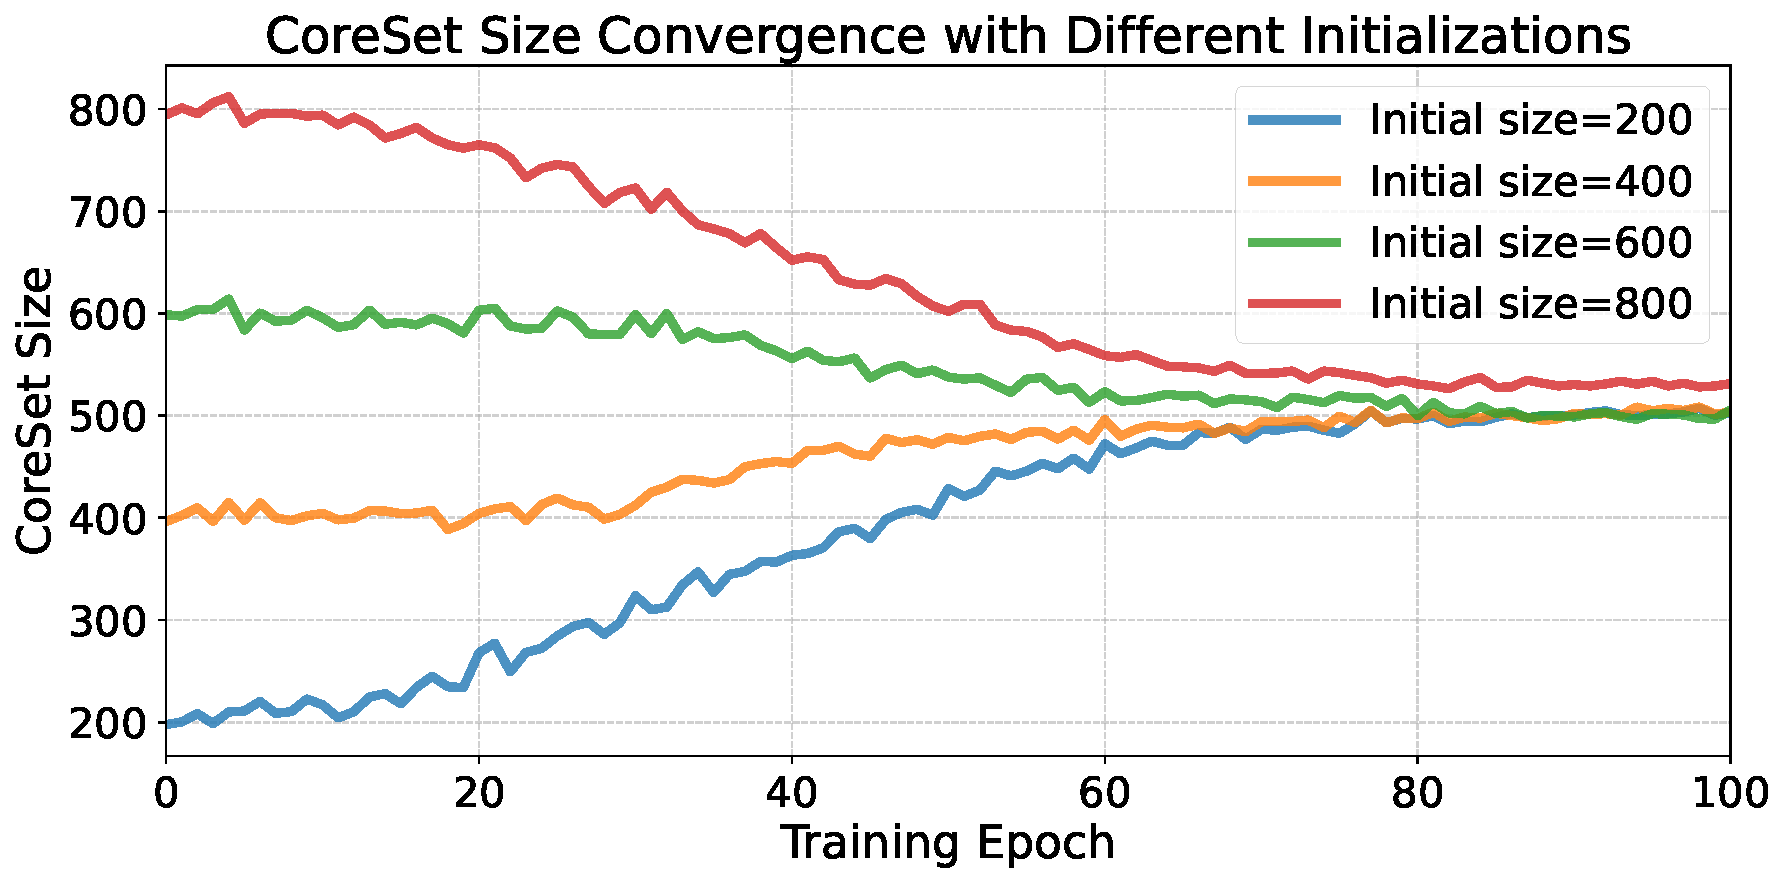
\includegraphics[width=\linewidth]{pics/coreset_convergence.pdf}
    \caption{Subset size evolution during optimization with Bilevel-CADS starting from different initial subset sizes. }
    \label{fig:bilevel-cads-subset-size}
  \end{minipage}%
  \hfill
  \begin{minipage}[c]{0.52\textwidth}
    \centering
    \captionof{table}{Accuracy (\%) comparison of different data selection methods with various initial subset sizes on MNIST.}
    \resizebox{\linewidth}{!}{%
    \begin{tabular}{@{}lccccc@{}}
      \toprule
      \multirow{2}{*}{Method} & \multicolumn{4}{c}{Initial subset size}                           & \multirow{2}{*}{Average} \\ \cmidrule(lr){2-5}
                              & 200            & 400            & 600            & 800            &                          \\ \midrule
      Random                  & 88.05          & 90.62          & 90.75          & 89.91          & 89.83                    \\
      PBCS                    & 89.81          & 92.14          & {\ul 92.64}    & {\ul 92.98}    & 91.89                    \\
      CADS-E                  & {\ul 91.48}    & {\ul 92.28}    & 92.34          & 92.90          & {\ul 92.25}              \\
      Bilevel-CADS            & \textbf{92.44} & \textbf{92.90} & \textbf{92.85} & \textbf{93.09} & \textbf{92.80}           \\ \bottomrule
    \end{tabular}}
    
    \label{tab:data-selection-results}
  \end{minipage}
\end{figure}

As shown in Table~\ref{tab:data-selection-results}, Bilevel-CADS consistently achieves the highest accuracy across all initial subset sizes, significantly outperforming random selection and other methods. Meanwhile, Figure~\ref{fig:bilevel-cads-subset-size} visualizes how the Bilevel-CADS optimization process converges to a stable subset size near 500 samples regardless of the initial subset size, indicating robustness and effective subset refinement driven by the compute budget constraint.


\subsection{Performance with heterogeneous data sources}
\label{sec:heter-ds}
\begin{figure}[!h]
  \centering
  \begin{minipage}[c]{0.48\textwidth}
    \centering
    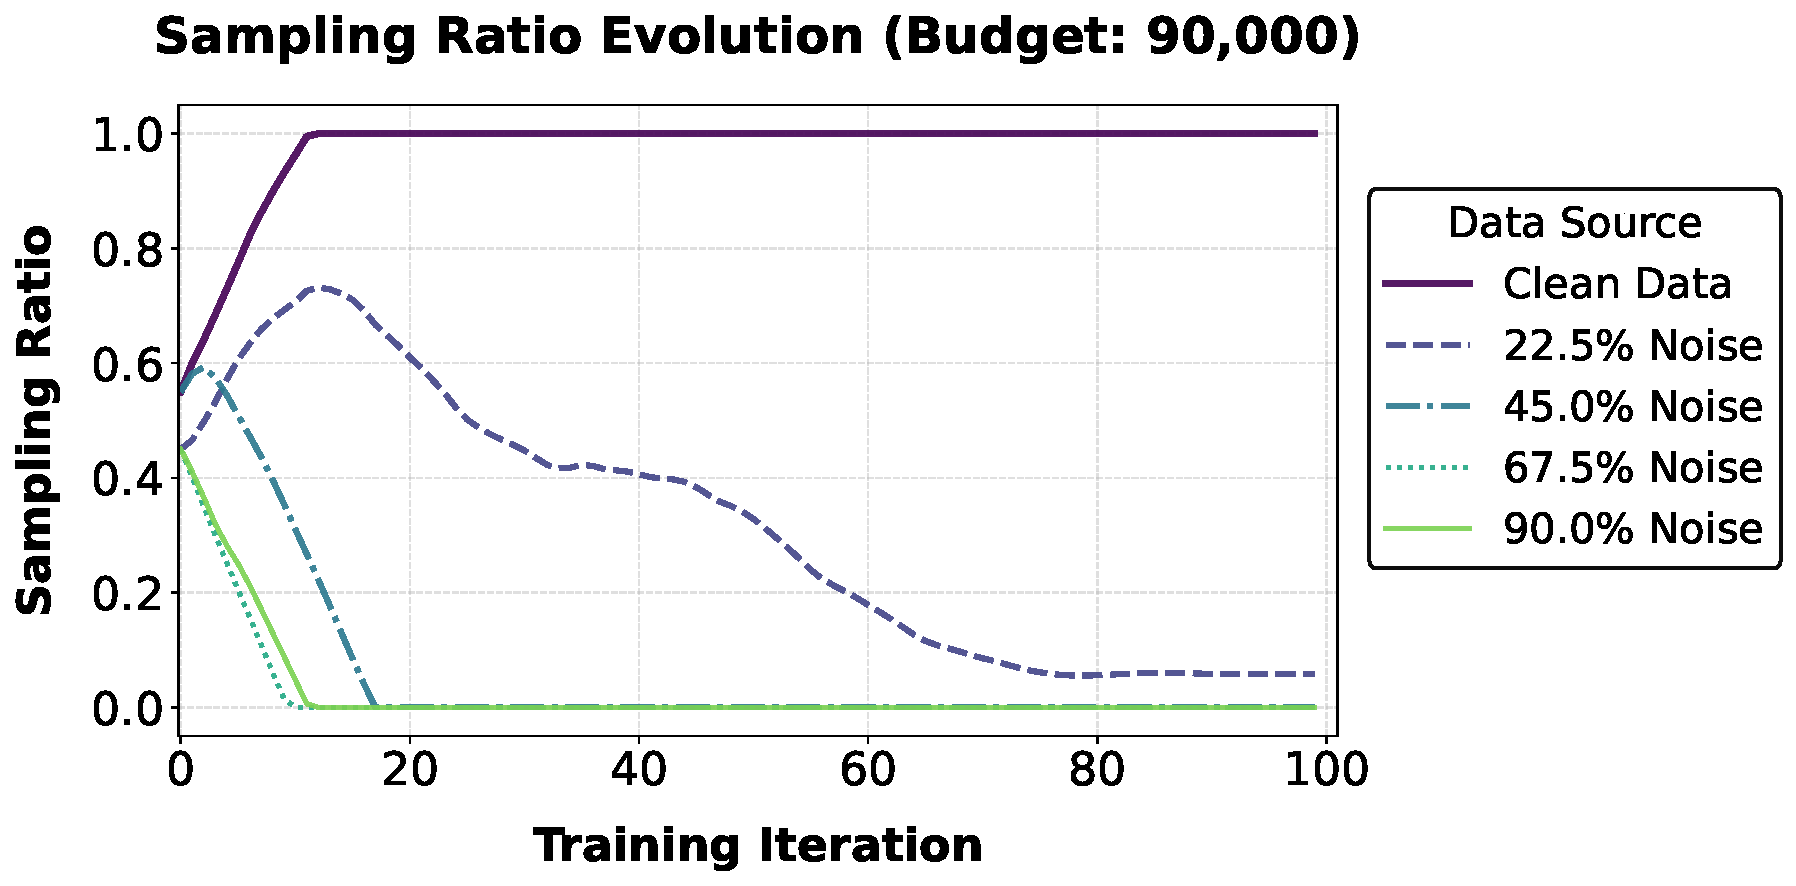
\includegraphics[width=\linewidth]{pics/sampling_ratio_evolution_ep2.pdf}
    % \caption{Sampling ratio evolution with a compute budget of 90,000}
    \label{fig:cads-s-cifar-s-ep2}
  \end{minipage}%
  \hfill
  \begin{minipage}[c]{0.48\textwidth}
    \centering
    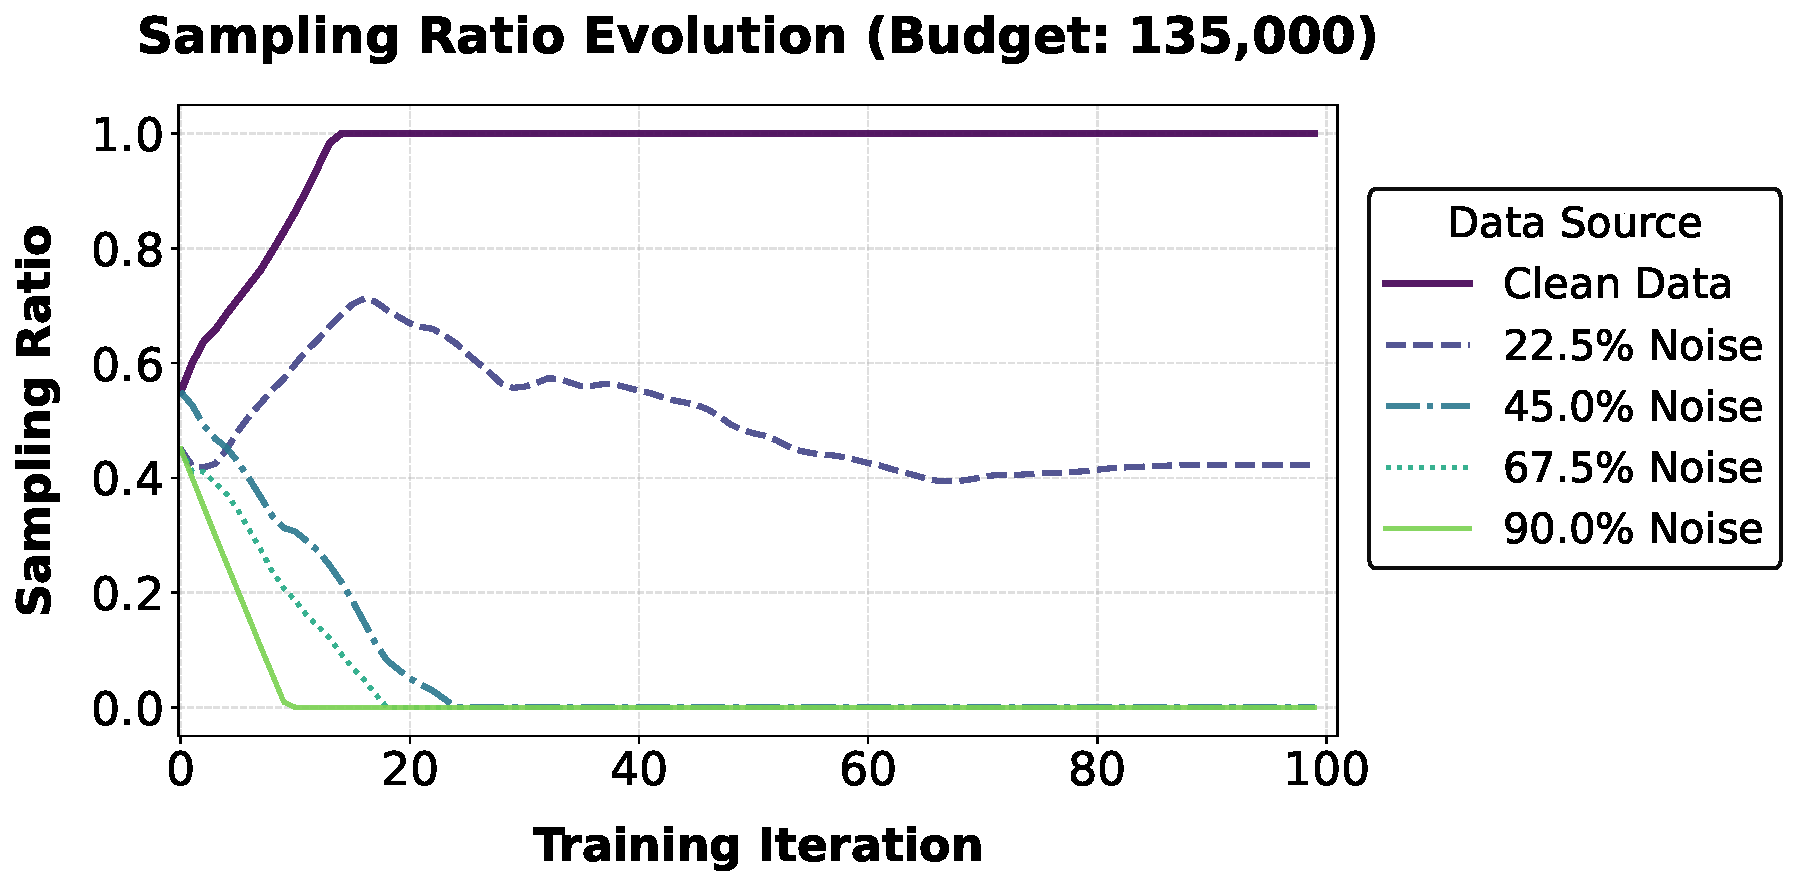
\includegraphics[width=\linewidth]{pics/sampling_ratio_evolution_ep3.pdf}
    % \caption{Sampling ratio evolution with a compute budget of 135,000}
    \label{fig:cads-s-cifar-s-ep3}
  \end{minipage}%
  % \hfill
  
  \begin{minipage}[c]{0.48\textwidth}
    \centering
    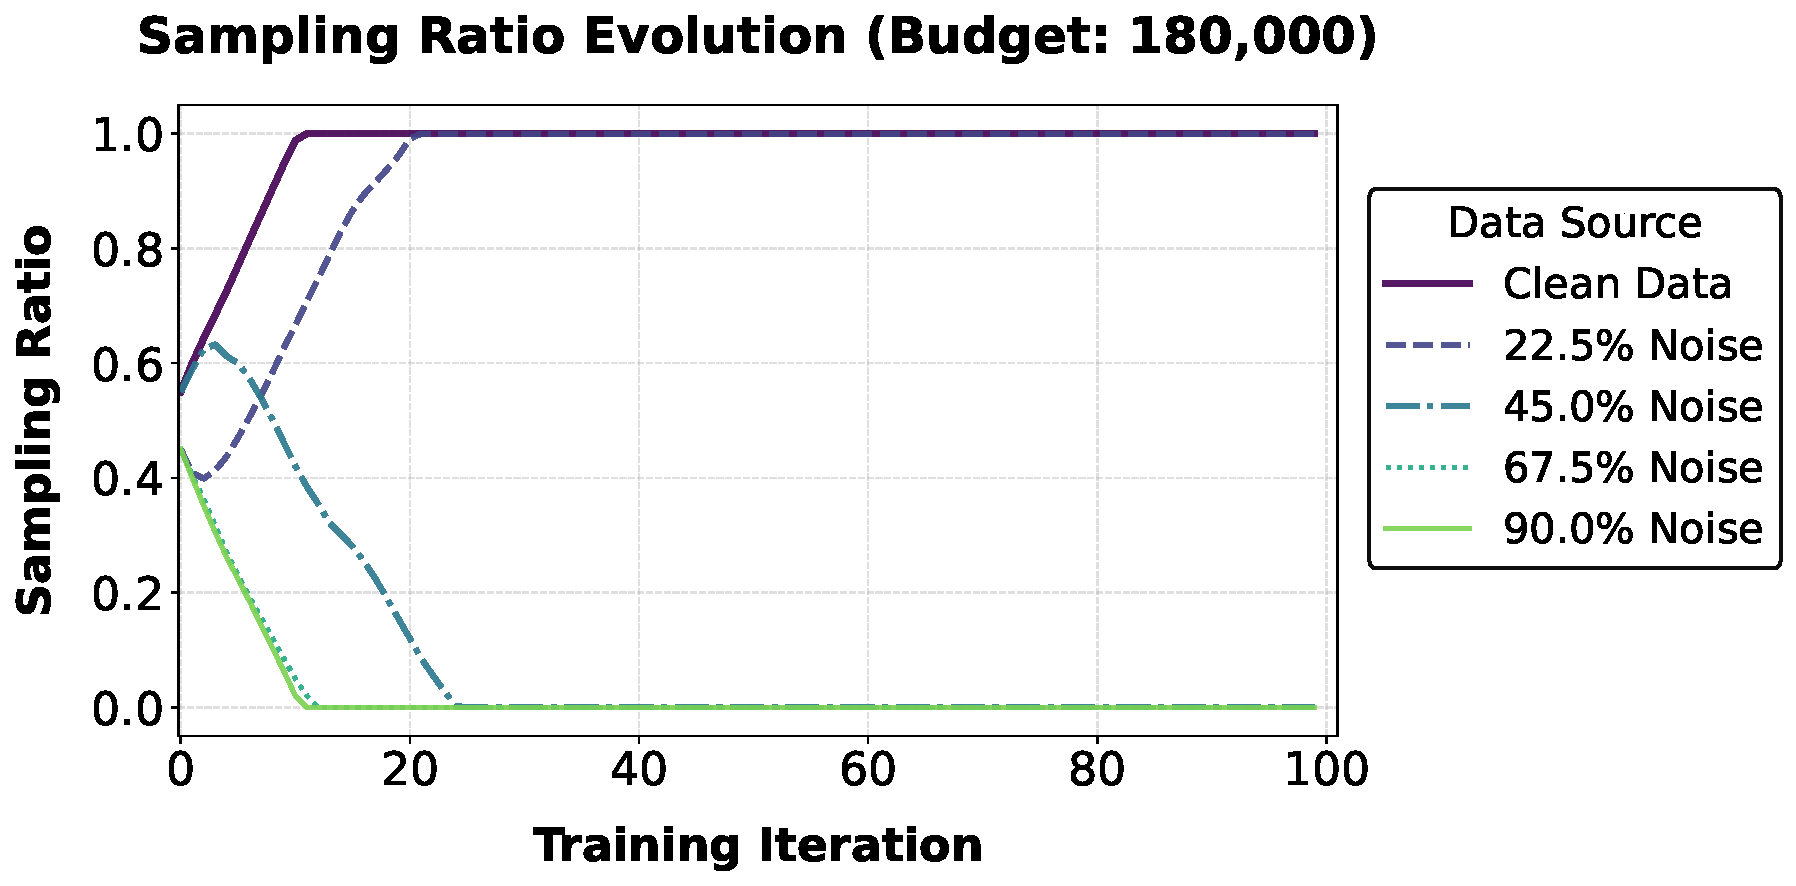
\includegraphics[width=\linewidth]{pics/sampling_ratio_evolution_ep4.pdf}
    % \caption{Sampling ratio evolution with a compute budget of 180,000}
    \label{fig:cads-s-cifar-s-ep4}
  \end{minipage}%
  \hfill
  \begin{minipage}[c]{0.48\textwidth}
    \centering
    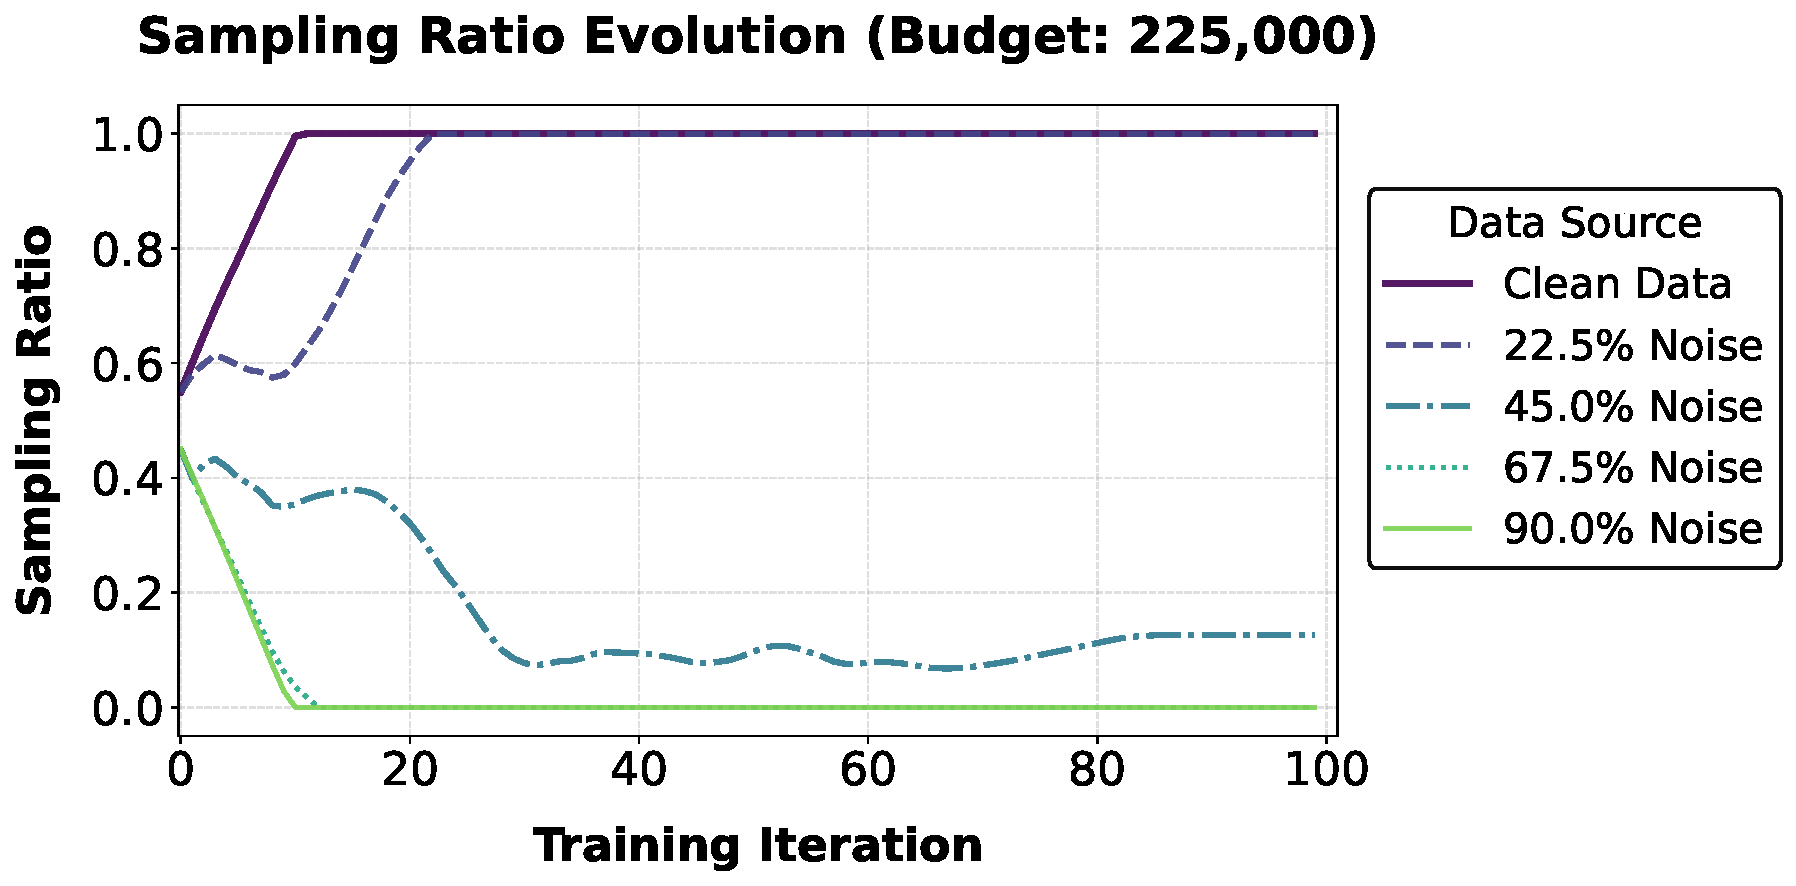
\includegraphics[width=\linewidth]{pics/sampling_ratio_evolution_ep5.pdf}
    % \caption{Sampling ratio evolution with a compute budget of 180,000}
    \label{fig:cads-s-cifar-s-ep5}
  \end{minipage}%
  \caption{Evolution of the sampling ratio over training iterations under different compute budgets: 90,000, 135,000, 180,000, and 225,000 samples respectively. }
  \label{fig:cads-sampling-ratio-evolution}
\end{figure}
\paragraph{Small-scale experiments on CIFAR-10.}
To validate the effectiveness of CADS-S, we conducted experiments on the CIFAR-10 dataset. Specifically, we reserved 10\% of the training set (5,000 samples) as a validation set and partitioned the remaining 45,000 samples into five equal groups of 9,000 each, simulating heterogeneous data sources with noise levels of 0\%, 22.5\%, 45.0\%, 67.5\%, and 90.0\%, respectively. Our objective was to assess how CADS-S performs compared to training on the single best data source, and the full dataset. The compute budget was varied between 90,000 and 225,000 sample usages.

\paragraph{Key Insights from Fig.~\ref{fig:cads-sampling-ratio-evolution}:}
It clearly illustrates that, under lower compute budgets, our algorithm predominantly favors clean data, assigning near-zero weights to the noisy data sources. However, with an increase in the compute budget, the algorithm gradually elevates the weights of data sources with lower noise levels.

At a compute budget of 225,000 samples, the algorithm incorporates both the clean data and data from the source with 22.5\% noise, while also selecting a negligible amount (<0.1) from the source with 45\% noise. This phenomenon highlights that as the compute budget expands, even data containing some noise can retain significant value in the training process.

In stark contrast, data sources with noise levels greater than 60\% are consistently excluded from selection, regardless of the compute budget in play. These findings suggest that as the compute budget grows, the algorithm becomes increasingly adept at leveraging noisy data, emphasizing the importance of diverse data sources in enhancing model performance.

\begin{figure}[!h]
  \centering
  \begin{minipage}[c]{0.48\textwidth}
    \centering
    \captionof{table}{Accuracy (\%) comparison of different data selection methods with various compute budget.}
    \resizebox{\linewidth}{!}{%
    \begin{tabular}{@{}lccccc@{}}
      \toprule
      \multirow{2}{*}{Method} & \multicolumn{4}{c}{Compute budget}                           & \multirow{2}{*}{Average} \\ \cmidrule(lr){2-5}
                              & 90,000            & 135,000            & 180,000            & 225,000            &                          \\ \midrule
      Best-source                  & 56.31          & 61.59          & 63.72         & 65.08          & 61.65                    \\
      Full-dataset                   & 44.34          & 49.80          & 53.34    & 57.03    & 51.13                    \\
      CADS-S            & \textbf{57.05} & \textbf{62.07} & \textbf{65.96} & \textbf{67.22} & \textbf{63.08}           \\ \bottomrule
    \end{tabular}}
    
    \label{tab:cads-s-cifar-results}
  \end{minipage}
  \hfill
  \begin{minipage}[c]{0.48\textwidth}
    \centering
    \captionof{table}{Accuracy (\%) comparison of different data selection methods with various initial subset sizes on DomainNet.}
    \resizebox{\linewidth}{!}{%
    \begin{tabular}{@{}lccccc@{}}
      \toprule
      \multirow{2}{*}{Method} & \multicolumn{4}{c}{Initial sampling ratio (\%)}                           & \multirow{2}{*}{Average} \\ \cmidrule(lr){2-5}
                              & 20            & 40            & 60            & 80            &                          \\ \midrule
      Uniform-sampling                  & 29.73          & 37.48          & 39.70          & 37.96          & 36.22                    \\
      CADS-S                  & \textbf{44.15}    & \textbf{44.22}    & \textbf{44.23}          & \textbf{44.49}          & \textbf{42.27}              \\ \bottomrule
    \end{tabular}}
    
    \label{tab:domainnet-results}
  \end{minipage}
\end{figure}

\paragraph{Scaling to larger datasets}  
To further evaluate the scalability and effectiveness of our approach, we conduct experiments on the DomainNet dataset~\cite{domainnet}, which contains over 0.5 million images across six diverse visual domains: Real, Sketch, Clipart, Painting, Infograph, and Quickdraw. Our setup uses all domains as data sources; however, we treat the Real domain as a high-quality data source and only include a subset of 10,000 samples from it to simulate limited access to the most reliable data. The other five domains are used in full.
The total compute budget allocated for training corresponds approximately to training on the full dataset for 10 epochs. 
Table~\ref{tab:domainnet-results} reports the test accuracy of different data selection methods under varying initial sampling ratios. Our proposed CADS-S method consistently improves over uniform sampling across all ratios.
Figure~\ref{fig:cads-s-domain-s-ep10} illustrates the evolution of sampling ratios during the optimization process, demonstrating how CADS-S dynamically adjusts data source importance over epochs to better allocate the computational budget.
\begin{figure}[!h]
  \centering
  \begin{minipage}[c]{0.54\textwidth}
    \centering
    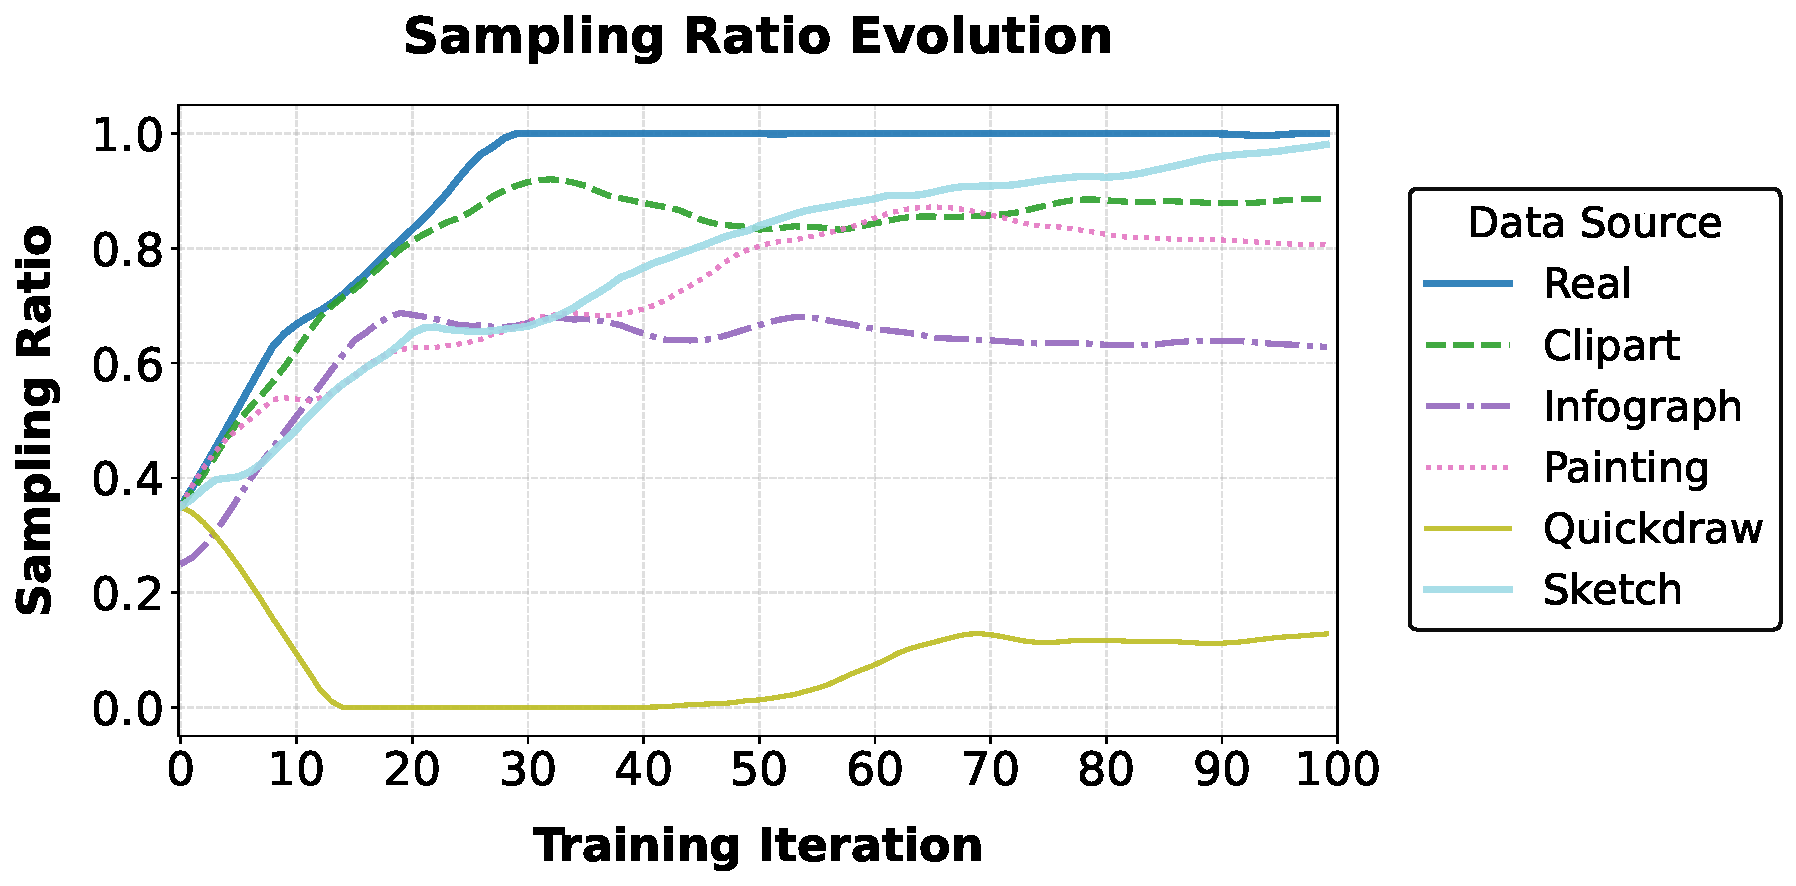
\includegraphics[width=\linewidth]{pics/sampling_ratio_evolution_extended.pdf}
    \caption{Sampling ratio evolution on DomainNet}
    \label{fig:cads-s-domain-s-ep10}
  \end{minipage}%
  \hfill
  \begin{minipage}[c]{0.38\textwidth}
    \centering
    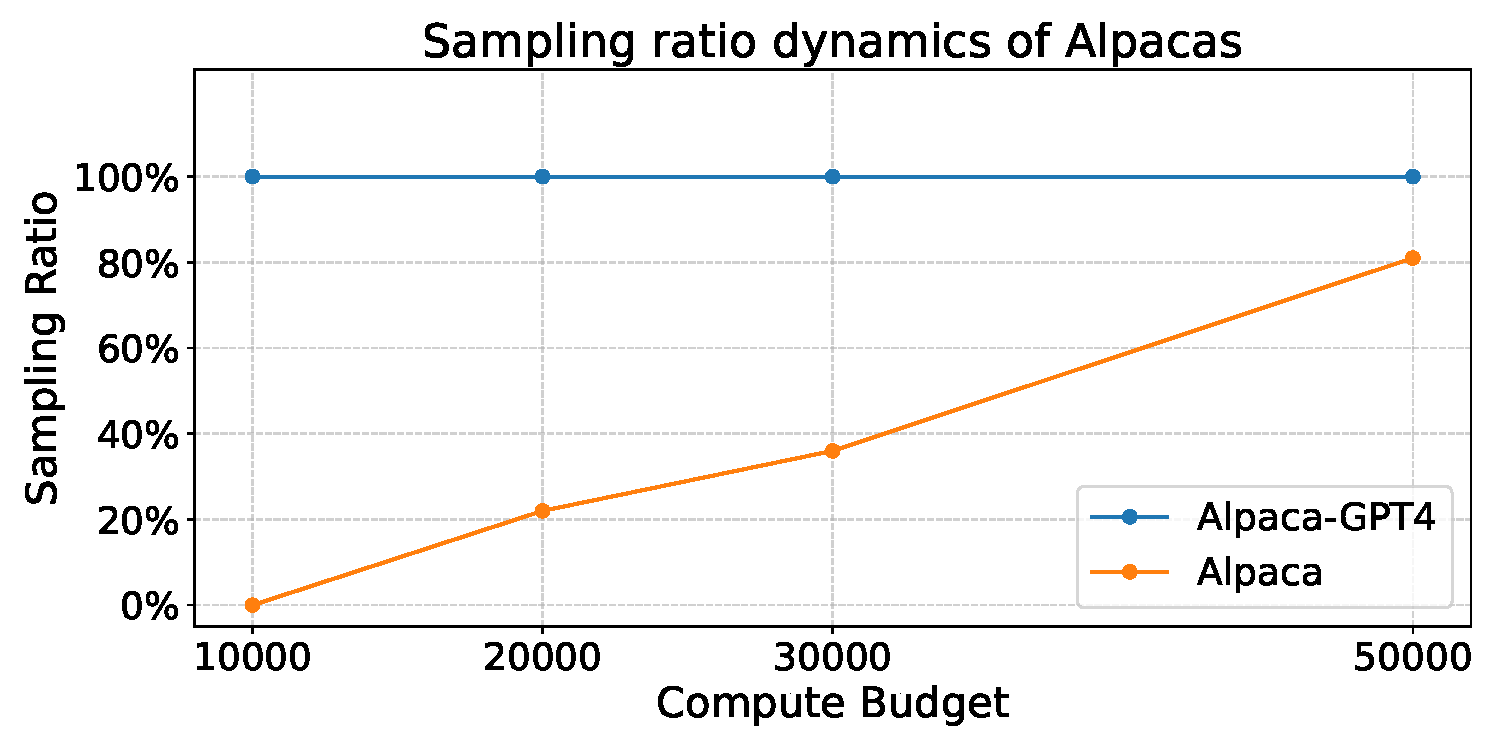
\includegraphics[width=\linewidth]{pics/sampling_ratio_dynamics.pdf}
    \caption{Sampling ratio dynamics of Alpaca-GPT4 and Alpaca datasets under different compute budgets optimized by CADS-S.}
    \label{fig:ratio-vs-budget-alpaca}
  \end{minipage}%
\end{figure}
\subsection{Performance on instruction tuning tasks}
\paragraph{Small-scale experiments.}
We evaluated our CADS-S approach on instruction fine-tuning tasks using the GPT-2 model~\cite{Radford2019LanguageMA}. The dataset consists of two heterogeneous data sources: (i) \textbf{Alpaca-GPT4}~\cite{alpaca-gpt4}, a high-quality dataset from GPT-4-generated instructions, from which we sample 1,000 examples to simulate the rarity of premium data sources in practical scenarios; (ii) \textbf{Alpaca}~\cite{alpaca}, a larger dataset containing 9,000 examples, representing standard quality data. The total compute budget varies within the range \([1 \times 10^{4}, 5 \times 10^{4}]\) sample usages. Other settings remain consistent with those described in Section~\ref{sec:heter-ds}. As shown in Tab~\ref{tab:cads-s-gpt2-results}, CADS-S consistently outperforms baseline methods, across all compute budgets studied. This validates the proposed method’s ability to allocate computational resources between heterogeneous data sources to optimize model performance. 

\paragraph{Scaling to additional datasets.}

\begin{figure}[!h]
  \centering
  \begin{minipage}[c]{0.38\textwidth}
    \centering
    \captionof{table}{Perplexity comparison of different data selection methods with various compute budget.}
    \resizebox{\linewidth}{!}{%
    \begin{tabular}{@{}lcccc@{}}
      \toprule
      \multirow{2}{*}{Method} & \multicolumn{4}{c}{Compute budget}                          \\ \cmidrule(lr){2-5}
                              & 1e+4            & 2e+4            & 3e+4            & 5e+4          \\ \midrule
      Best-source                  & 8.01          & 8.02          & 8.21         & 8.87         \\
      Full-dataset                   & 8.26          & 8.01          & 7.90    & 7.77                    \\
      CADS-S            & \textbf{8.01} & \textbf{7.92} & \textbf{7.85} & \textbf{7.77}         \\ \bottomrule
    \end{tabular}
    }
    
    \label{tab:cads-s-gpt2-results}
  \end{minipage}
  \hfill
  \begin{minipage}[c]{0.58\textwidth}
    \centering
    \captionof{table}{Perplexity comparison of different data selection methods with various initial subset sizes on additional datasets.}
    \resizebox{\linewidth}{!}{%
    \begin{tabular}{@{}lccccc@{}}
      \toprule
      \multirow{2}{*}{Method} & \multicolumn{4}{c}{Initial sampling ratio (\%)}                           & \multirow{2}{*}{Average} \\ \cmidrule(lr){2-5}
                              & 20            & 40            & 60            & 80            &                          \\ \midrule
      Uniform-sampling                  & 7.90          & 7.52          & 7.43          & 7.39          & 7.56                    \\
      CADS-S                  & \textbf{6.97}    & \textbf{6.95}    & \textbf{6.97}          & \textbf{6.90}          & \textbf{6.95}              \\ \bottomrule
    \end{tabular}}
    
    \label{tab:additional}
  \end{minipage}
\end{figure}

We further evaluated CADS across 13 instruction-following fine-tuning datasets, sampling 10,000 examples from each, including AlpacaGPT4~\cite{alpaca-gpt4}, SlimOrca~\cite{slimorca}, Alpaca~\cite{alpaca}, GPTeacher~\cite{gpteacher}, and multilingual Alpaca variants, totaling around 130,000 samples. Detailed dataset setups and preprocessing are provided in the appendix.  
As shown in Tab~\ref{tab:additional}, our method consistently outperforms baseline approaches in perplexity across different initial sampling ratios, demonstrating its robustness and wide applicability.  

\subsection{Computational Cost Analysis of Established Baselines}

To provide a clear comparison of computational efficiency, we establish a unified framework parameterized by: 
\begin{itemize}
    \item \textbf{C}: The total compute budget required for a single, standard training run on the full dataset. This serves as our baseline unit of cost.
    \item \textbf{N}: The total number of samples in the full dataset.
    \item \textbf{T}: The number of training epochs, defined as $T = C/N$.
\end{itemize}
All computational overheads are measured relative to the baseline cost \textbf{C} of training on the full dataset.

\textbf{A Note on Pre-training Cost:} For methods that require a pre-trained model to compute sample-wise statistics (e.g., gradients, forgetting events), we assume the cost of obtaining this model is **0.2C**. This represents a standard approximation for the early-stage training necessary to yield meaningful statistics, without requiring full convergence.

\begin{table}[h!]
\centering
\caption{Computational Cost Analysis of Established Baselines.}
\label{tab:cost_analysis}
\resizebox{\linewidth}{!}{%
\begin{tabular}{@{}ll@{}}
\toprule
\textbf{Method} & \textbf{Total Computational Overhead} \\
\midrule
Random Selection & C (no additional cost) \\
Forgetting Scores & 1.2C (0.2C for pre-training and forgetting computation + C for final training) \\
GraNd & 1.2C (0.2C for pre-training and gradient computation + C for final training) \\
EL2N & 1.2C (0.2C for pre-training and error computation + C for final training) \\
CADS (Ours) & $(5/A + 2\gamma)\text{C where A is amortization factor}$ \\
Influence Functions & $2\text{C} + O(N^2)$ (full training + expensive Hessian computations + final training) \\
Data Shapley & 11C--101C (C for final training + 10C--100C for Monte Carlo approximation) \\
Probabilistic Bilevel Optimization & 50C--100C (requires 50--100 outer iterations) \\
Greedy Coreset & $\sim(N^2/T+1)\text{C where K is coreset size}$ \\
\bottomrule
\end{tabular}}
\end{table}

\textbf{Summary:} CADS achieves superior efficiency among bilevel methods with overhead $(5/A + 2\gamma)\text{C}$. With A=5 amortization, total cost reduces to $2\gamma\text{C}$, $\gamma < 1$. Traditional methods like Forgetting Scores offer moderate 1.2C cost but lack budget-aware optimization and deliver inferior effectiveness. Advanced bilevel methods become prohibitively expensive (50C+), while CADS provides an optimal balance between computational efficiency and budget-aware capabilities.

\textbf{Note:} The core contribution of our work is introducing computational budget constraints into coreset selection, rather than optimizing selection time alone. Once learned, a coreset can be reused multiple times across different training scenarios, model architectures, and experiments. Therefore, the computational investment in coreset selection can be amortized over multiple uses, making the selection efficiency a secondary consideration compared to the quality of the resulting coreset under budget constraints.
